% !TeX spellcheck = en_GB
% !TeX encoding = UTF-8
% !TeX program = xelatex
% TODO Change language to en_GB (recommended) or en_US for English documents
\documentclass[11pt,a4paper,oneside]{report}             % Single-side
%\documentclass[11pt,a4paper,twoside,openright]{report}  % Duplex

% thanks to http://tex.stackexchange.com/a/47579/71109
\usepackage{ifxetex}
\usepackage{ifluatex}
\newif\ifxetexorluatex % a new conditional starts as false
\ifnum 0\ifxetex 1\fi\ifluatex 1\fi>0
   \xetexorluatextrue
\fi

\ifxetexorluatex
  \usepackage{fontspec}
\else
  \usepackage[T1]{fontenc}
  \usepackage[utf8]{inputenc}
  \usepackage[lighttt]{lmodern}
\fi

\usepackage[english,magyar]{babel} % Alapértelmezés szerint utoljára definiált nyelv lesz aktív, de később külön beállítjuk az aktív nyelvet.

%\usepackage{cmap}
\usepackage{amsfonts,amsmath,amssymb} % Mathematical symbols.
%\usepackage[ruled,boxed,resetcount,linesnumbered]{algorithm2e} % For pseudocodes. % beware: this is not compatible with LuaLaTeX, see http://tex.stackexchange.com/questions/34814/lualatex-and-algorithm2e
\usepackage{booktabs} % For publication quality tables for LaTeX
\usepackage{graphicx}


%\usepackage{fancyhdr}
%\usepackage{lastpage}
\usepackage{float}
\usepackage{anysize}
\usepackage{wrapfig}
%\usepackage{sectsty}
\usepackage{setspace} % For setting line spacing

\PassOptionsToPackage{hyphens}{url}\usepackage{hyperref}
\usepackage{xcolor}
\usepackage{listings} % For source code snippets.

\usepackage[amsmath,thmmarks]{ntheorem} % Theorem-like environments.

\usepackage[hang]{caption}

\singlespacing

\newcommand{\sectionbreak}{\clearpage}

\newcommand{\selecthungarian}{
	\selectlanguage{magyar}
	\setlength{\parindent}{2em}
	\setlength{\parskip}{0em}
	\frenchspacing
}

\newcommand{\selectenglish}{
	\selectlanguage{english}
	\setlength{\parindent}{0em}
	\setlength{\parskip}{0.5em}
	\nonfrenchspacing
	\renewcommand{\figureautorefname}{Figure}
	\renewcommand{\tableautorefname}{Table}
	\renewcommand{\partautorefname}{Part}
	\renewcommand{\chapterautorefname}{Chapter}
	\renewcommand{\sectionautorefname}{Section}
	\renewcommand{\subsectionautorefname}{Section}
	\renewcommand{\subsubsectionautorefname}{Section}
}

\usepackage[numbers]{natbib}
\usepackage{xspace}


%TODO Set the main variables
\newcommand{\vikszerzoVezeteknev}{Maidics}
\newcommand{\vikszerzoKeresztnev}{Barnabas}

\newcommand{\vikkonzulensAMegszolitas}{}
\newcommand{\vikkonzulensAVezeteknev}{Vary}
\newcommand{\vikkonzulensAKeresztnev}{Peter}

\newcommand{\vikkonzulensBMegszolitas}{dr.~}
\newcommand{\vikkonzulensBVezeteknev}{Dudas}
\newcommand{\vikkonzulensBKeresztnev}{Akos}

\newcommand{\vikkonzulensCMegszolitas}{}
\newcommand{\vikkonzulensCVezeteknev}{}
\newcommand{\vikkonzulensCKeresztnev}{}

\newcommand{\vikcim}{Hive performance analysis and optimization} % Cím
\newcommand{\viktanszek}{Department of Automation and Applied Informatics} % Tanszék
\newcommand{\vikdoktipus}{\bsc} % Dokumentum típusa (\bsc vagy \msc)
\newcommand{\vikmunkatipusat}{szakdolgozatot} % a "hallgató nyilatkozat" részhez: szakdolgozatot vagy diplomatervet

\input{include/tdk-variables}
\newcommand{\szerzoMeta}{\vikszerzoVezeteknev{} \vikszerzoKeresztnev} % egy szerző esetén
%\newcommand{\szerzoMeta}{\vikszerzoVezeteknev{} \vikszerzoKeresztnev, \tdkszerzoB} % két szerző esetén

%TODO Language configuration -- choose one
% Beállítások magyar nyelvű dolgozathoz
%\input{include/thesis-hu}
% Settings for English documents
%--------------------------------------------------------------------------------------
% Elnevezések
%--------------------------------------------------------------------------------------
\newcommand{\bme}{Budapest University of Technology and Economics}
\newcommand{\vik}{Faculty of Electrical Engineering and Informatics}

\newcommand{\bmemit}{Department of Measurement and Information Systems}

\newcommand{\keszitette}{Author}
\newcommand{\konzulens}{Advisors}

\newcommand{\bsc}{Bachelor's Thesis}
\newcommand{\msc}{Master's Thesis}
\newcommand{\tdk}{Scientific Students' Association Report}
\newcommand{\bsconlab}{BSc Project Laboratory}
\newcommand{\msconlabi}{MSc Project Laboratory 1}
\newcommand{\msconlabii}{MSc Project Laboratory 2}

\newcommand{\pelda}{Example}
\newcommand{\definicio}{Definition}
\newcommand{\tetel}{Theorem}

\newcommand{\bevezetes}{Introduction}
\newcommand{\koszonetnyilvanitas}{Acknowledgements - Köszönetnyilvánítás}
\newcommand{\fuggelek}{Appendix}

% Optional custom titles
%\addto\captionsenglish{%
%\renewcommand*{\listfigurename}{Your list of figures title}
%\renewcommand*{\listtablename}{Your list of tables title}
%\renewcommand*{\bibname}{Your bibliography title}
%}

\newcommand{\szerzo}{\vikszerzoKeresztnev{} \vikszerzoVezeteknev}
\newcommand{\vikkonzulensA}{\vikkonzulensAMegszolitas\vikkonzulensAKeresztnev{} \vikkonzulensAVezeteknev}
\newcommand{\vikkonzulensB}{\vikkonzulensBKeresztnev{} \vikkonzulensBVezeteknev, \vikkonzulensBMegszolitas}
\newcommand{\vikkonzulensC}{\vikkonzulensCMegszolitas\vikkonzulensCKeresztnev{} \vikkonzulensCVezeteknev}

\newcommand{\selectthesislanguage}{\selectenglish}

\bibliographystyle{plainnat}

\newcommand{\ie}{i.e.\@\xspace}
\newcommand{\Ie}{I.e.\@\xspace}
\newcommand{\eg}{e.g.\@\xspace}
\newcommand{\Eg}{E.g.\@\xspace}
\newcommand{\etal}{et al.\@\xspace}
\newcommand{\etc}{etc.\@\xspace}
\newcommand{\vs}{vs.\@\xspace}
\newcommand{\viz}{viz.\@\xspace} % videlicet
	\newcommand{\cf}{cf.\@\xspace} % confer
\newcommand{\Cf}{Cf.\@\xspace}
\newcommand{\wrt}{w.r.t.\@\xspace} % with respect to
\newcommand{\approximately}{approx.\xspace}

\newcommand{\appendixnumber}{1}  % a fofejezet-szamlalo az angol ABC 1. betuje (A) lesz


\input{include/preamble}

%--------------------------------------------------------------------------------------
% Table of contents and the main text
%--------------------------------------------------------------------------------------
\begin{document}

%TODO These define guidelines -- remove these
%~~~~~~~~~~~~~~~~~~~~~~~~~~~~~~~~~~~~~~~~~~~~~~~~~~~~~~~~~~~~~~~~~~~~~~~~~~~~~~~~~~~~~~
%\include{include/guideline}
%\include{include/project}

\selectthesislanguage

%TODO Titlepage -- choose one from below
%~~~~~~~~~~~~~~~~~~~~~~~~~~~~~~~~~~~~~~~~~~~~~~~~~~~~~~~~~~~~~~~~~~~~~~~~~~~~~~~~~~~~~~
\include{include/titlepage}		   % Szakdolgozat/Diplomaterv címlap
%\include{include/titlepage-tdk}	% TDK címlap
%\include{include/titlepage-otdk}   % OTDK címlap


% Table of Contents
%~~~~~~~~~~~~~~~~~~~~~~~~~~~~~~~~~~~~~~~~~~~~~~~~~~~~~~~~~~~~~~~~~~~~~~~~~~~~~~~~~~~~~~
\tableofcontents\vfill


% Declaration and Abstract
%~~~~~~~~~~~~~~~~~~~~~~~~~~~~~~~~~~~~~~~~~~~~~~~~~~~~~~~~~~~~~~~~~~~~~~~~~~~~~~~~~~~~~~
\include{include/declaration} %TODO Hallgatói nyilatkozat -- TDK és OTDK esetén törlendő!
\pagenumbering{roman}
\setcounter{page}{1}

\selecthungarian

%----------------------------------------------------------------------------
% Abstract in Hungarian
%----------------------------------------------------------------------------
\chapter*{Kivonat}\addcontentsline{toc}{chapter}{Kivonat}

Apache Hive eredetileg a Facebook által készített nyílt forráskódú, adattárház platform. Célja, hogy megkönnyítse az adatelemzők munkáját azzal, hogy bevezetett egy, az SQL-hez hasonló nyelvet, a HiveQL-t. Hive bemenete egy HiveQL lekérdezés, amit feldolgoz, szemantikailag elemzi, majd amennyiben lehetséges optimalizálja különböző optimalizációs stratégiákat felhasználva. Végezetül generál egy Hadoop feladatot, amit az végre tud hajtani. Hive nem csak Hadoopot tud használni végrehajtó motortként, támogatja az Apache Spark és Apache Tez használatát is. 

Bizonyos körülmények között Hive memória problémákkal küzd. HiveServer2 az egyik fő komponense, gyakran összeomlik Out Of Memory (OOM) hibaüzenettel. Jelen dolgozattal a célom, hogy felépítsek egy alapvető modellt, melnyek segítségével megtudjuk miért és a lekérdezés életciklusában mikor növekszik jelentősen a memóriahasználat, valamint memória problémákat találjak és amennyiben lehetséges ezekre megoldási javaslatot adjak.

A model építéshez segítségül létrehoztam egy eszközt, melynek használatával információkat tudok kinyerni a memóriahasználattal kapcsolatban és heap mintákat (heap dump) tudok generálni automatikusan a lekérdezés élete során, későbbi elemzés céljából. Az említett és más memória elemző eszközök segítségével azonosítottam két problémát, amik a heap memóriát jelentősen tudják növelni. Az egyik probléma HDFS-ből származik (Hadoop elosztott fájlrendszere), ezért Hadoop kód megértése és módosítása is szükségessé vált. Mindkét memória problémára, létrehoztam egy megoldási javaslatot, és csináltam egy lehetséges implementációt ami segíthet megszabadulni a memória problémától. Mindkét javítás alapos tesztelést igényelt: lokális, egyszerű teljesítmény tesztekre és skálázható adatközpont klaszteren végrehajtott benchmark tesztekre is szükség volt. Az azonosított problémák vizsgálata jelenleg is folyamatban van. A HDFS javításom előidézhet nehezen detektálható, váratlan CPU problémákat, ezért annak eldöntésére hogy a kompromisszum előnyös lesz, nagyon alapos tesztelés szükséges.


\vfill
\selectenglish


%----------------------------------------------------------------------------
% Abstract in English
%----------------------------------------------------------------------------
\chapter*{Abstract}\addcontentsline{toc}{chapter}{Abstract}
Apache Hive is an open source data warehouse platform originally built on top of Hadoop by Facebook. Hive makes the work of data scientists easier by introducing a language similar to SQL, called HiveQL. Hive takes query written in HiveQL, does parsing and analyzing and if possible, optimizes the query using several optimization strategies. Finally, it creates a Hadoop job and executes it on the platform. Currently, not only Hadoop can be used as an execution engine, Hive can even work on Apache Spark or Apache Tez. 

Hive faces memory problems under certain circumstances. HiveServer2 is one of the main components of Hive and often crashes due to Out Of Memory (OOM) error. In my thesis, I aim to build a basic model, to understand why and when the memory usage of HiveServer2 rises and find memory-related problems or wastes.

To be able to build a model, I created a basic tool for getting memory information and generating heap dumps automatically during the life of a query. With the help of my tool and other memory analysis tools, I generated and analyzed many heap dumps. I was able to identify two issues that can cause big pressure on heap memory. One of the issues is introduced by HDFS (distributed file system of Hadoop), therefore touching Hadoop was also necessary. For both memory issues, I suggested a possible solution and created an implementation, that can help get rid of the memory overheads. These patches required multiple tests: local, simple performance testing and scalable benchmarking on a data center cluster. The issues identified are still ongoing and currently under investigation since the HDFS patch might introduce unexpected CPU overhead which are hard to detect so deciding whether this tradeoff is negligible requires a thorough testing. 

\vfill
\selectthesislanguage

\newcounter{romanPage}
\setcounter{romanPage}{\value{page}}
\stepcounter{romanPage}    %TODO Összefoglaló -- TDK és OTDK esetén nem kötelező


% The main part of the thesis
%~~~~~~~~~~~~~~~~~~~~~~~~~~~~~~~~~~~~~~~~~~~~~~~~~~~~~~~~~~~~~~~~~~~~~~~~~~~~~~~~~~~~~~
\pagenumbering{arabic}

%TODO import your own content
%----------------------------------------------------------------------------
\chapter{\bevezetes}
%----------------------------------------------------------------------------


The digital era has led to large amounts of data being amassed by companies every day. Data comes from multiple sources: sensors, sales data, communication systems, logging of system events \etc. According to Forbes \cite{Forbes} 2.5 quintillion bytes of data is created each day. That means 2.5 million Terabytes per day. Bigger corporations can easily create hundreds of Terabytes daily. We need a new solution to process this amount of data. The traditional relational databases (RDBMS) can deal only with Gigabytes. Hadoop provides a software framework to scale up our system for storing, processing and analyzing big data.

In this chapter, I will write about the basics of Hadoop architecture, why Hive was created on top of it and the performance issues it faces.

\section{Hadoop basics}
Apache Hadoop is an open source distributed framework for managing, processing  and storing a huge amount of data in clustered systems built from commodity hardware. All modules in Hadoop were designed with an assumption that hardware failures are frequent and should be automatically handled by the framework. One of the most important characteristics of Hadoop is that it partitions the data and computation across many hosts and executes computation in parallel close to the data it uses.  \cite{Hadoop-wiki}

The base of the Hadoop framework contains the following modules:
\begin{itemize}
	\item HDFS - Hadoop Distributed File System: designed to store large data sets reliably and stream those at high bandwidth to user applications.
	\item Hadoop MapReduce: an implementation of the MapReduce programming model for large data processing
	\item YARN - Yet Another Resource Negotiator: a resource management and job scheduling technology
	\item Hadoop Common: contains libraries and utilities for other Hadoop modules
\end{itemize}
\iffalse\subsection{Hadoop \vs traditional databases}
Traditional databases cannot be used when we want to process and store big data. Main differences between Hadoop and traditional RDBMS \cite{Hadoop-vs-RDBMS}:
\begin{itemize}
	\item \textbf{Data Volume}: RDBMS works better when data volume is low (Gigabytes). However, when data size is huge (Terabytes-Petabytes) traditional databases fail. Users have to pick another solution for the problem. Hadoop can easily handle this amount of data so it became the number one big data platform.
	\item \textbf{Data Variety}: It means what type of data we want to process. Hadoop is able to store and process either structured, semi-structured or unstructured data. Even though  it is mostly used for huge amounts of unstructured data. 
	In contrast, traditional RDBMS can only be used to manage structured or semi-structured data. 
	\item \textbf{Scalability}: RDBMS provides vertical scalability. We can add more resources, memory or CPU to a machine in the cluster. Whereas Hadoop scales horizontally which means we can add more machines to an existing cluster. As a result of this, Hadoop becomes fault tolerant. We can easily recover data in case of a failure.
	\item \textbf{Data Processing}: Apache Hadoop supports OLAP (Online Analytical Processing), which involves very complex queries and aggregations. The database design is de-normalized, having fewer tables. On the other hand, RDBMS supports OLTP (Online Transaction Processing), which involves fast query processing. The database design is normalized and contains large numbers of tables.
\end{itemize}\fi
\subsection{HDFS - Hadoop Distributed File System}
HDFS is the file system of Hadoop. It stores file system metadata and application data separately. The dedicated server that stores metadata is the NameNode. Application data is stored on other servers (DataNodes). These servers are connected and they communicate using TCP-based protocols \cite{Shvachko:2010:HDF:1913798.1914427}. 

The file system is based on the following goals and principles \cite{HDFS-docs}:
\begin{itemize}
	\item \textbf{Hardware failure}: Hardware failures should be considered as normal, rather than an exception. An HDFS instance consists of hundreds or thousands of components so this means that some of them will always be non-functional. Therefore, fault detection and automatic recovery is a must.
	\item \textbf{Streaming Data Access}: HDFS was designed for batch processing rather than interactive use. Therefore, HDFS users need streaming access to their data. This means that high throughput is more important than low latency.
	\item \textbf{Large Data Sets}: The size of a typical HDFS file is gigabytes to terabytes. Thus, the file system is tuned to support large files. 
	\item \textbf{Simple Coherency}: HDFS follows WORM (Write-Once-Read-Many) model. A file, once written should not be changed except for appends and truncates.  This assumption simplifies data coherency issues. A MapReduce application fits perfectly for this model.
	\item \textbf{Moving computation}: A computation is much more efficient if it is executed near the data it operates on. It is especially true for big data. 
	\item \textbf{Portability}: HDFS was designed to port from one platform to another with ease. 
\end{itemize}
\subsubsection*{NameNode}
NameNode keeps the directory tree of all files in the file system and tracks where data is kept across the cluster, it does not store the files. Clients talk to the NameNode whenever they want to locate a file. The NameNode's response is a list of relevant DataNode servers where the data is available. 

As a result of this approach, the NameNode is a Single Point of Failure in the HDFS cluster. Whenever the NameNode goes down, the file system becomes offline.
\begin{figure}[H]
	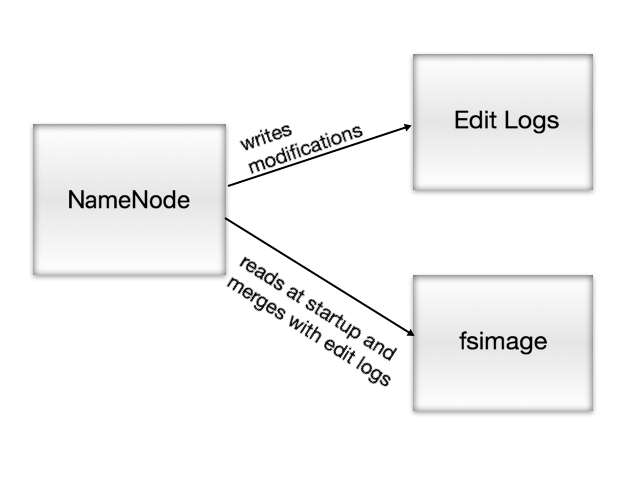
\includegraphics[width=80mm, keepaspectratio]{figures/namenode_problem.png}
	\centering
	\caption*{Problem with NameNode}
\end{figure}
The image shows how NameNode stores information \cite{Secondary-NameNode}. There are two different files:
\begin{itemize}
	\item edit logs: the changes made to the file system after the NameNode started
	\item fsimage: a snapshot of the file system when the NameNode started
\end{itemize}
In production clusters, the NameNode restarts are very rare. That means edit logs can grow large therefore in case of a crash we will lose a huge amount of metadata since the fsimage is very old.

The Secondary NameNode helps to solve this issue. It is responsible for merging the edit logs with fsimage. It collects edit logs on a regular basis and applies them to the fsimage. NameNode will use this fsimage in case of a crash and it can also be used to reduce the startup time of the NameNode.
It is important to remember that the Secondary NameNode is not a real backup NameNode it only merges the edits into the fsimage. 

\begin{figure}[H]
	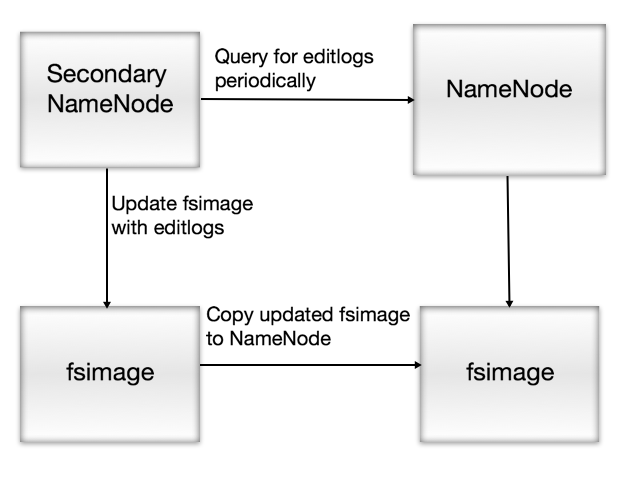
\includegraphics[width=80mm, keepaspectratio]{figures/secondary_namenode.png}
	\centering
	\caption*{Solution using the Secondary NameNode}
\end{figure}

\subsubsection*{DataNodes \cite{Shvachko:2010:HDF:1913798.1914427}}
On a DataNode, a block is represented by two files in the native file system. The first contains the data itself, the second is the metadata.

On startup, the DataNodes connect to the NameNode and perform a handshake. This will verify the namespace ID and software version of the DataNodes. If one of them does not match with the NameNode's value, the DataNode automatically shuts down. After a successful handshake, the DataNode registers with the NameNode. DataNode will store it's internal identifier. If restart occurs the DataNodes will be recognizable with the ID, even if they get a different IP address or port. After the ID is registered to the NameNode the it will never change. 

 When a DataNode is registered it sends a block report immediately. It contains block id, generation stamp and the length of each block the DataNode hosts. To provide up-to-date information to the NameNode reports are sent every hour. 

DataNodes send heartbeats to the NameNode. It ensures the NameNode that the DataNode is operating and block replicas of the server are available. If the NameNode does not receive a heartbeat from a DataNode it will consider the node to be out of service. The default heartbeat interval is three seconds.

\subsubsection*{HDFS Client \cite{Shvachko:2010:HDF:1913798.1914427}}
User applications can access the file system using the HDFS client which exports the HDFS file system interface. HDFS supports operations similar to a traditional file system: read, write, create or delete files and create or delete directories. The user can refer to files or directories using paths in the namespace.

When someone reads a file, HDFS Client asks the NameNode for the list of DataNodes that host replicas of the blocks of the file. Then it will directly contact the DataNode and request the desired block.

\begin{figure}[H]
	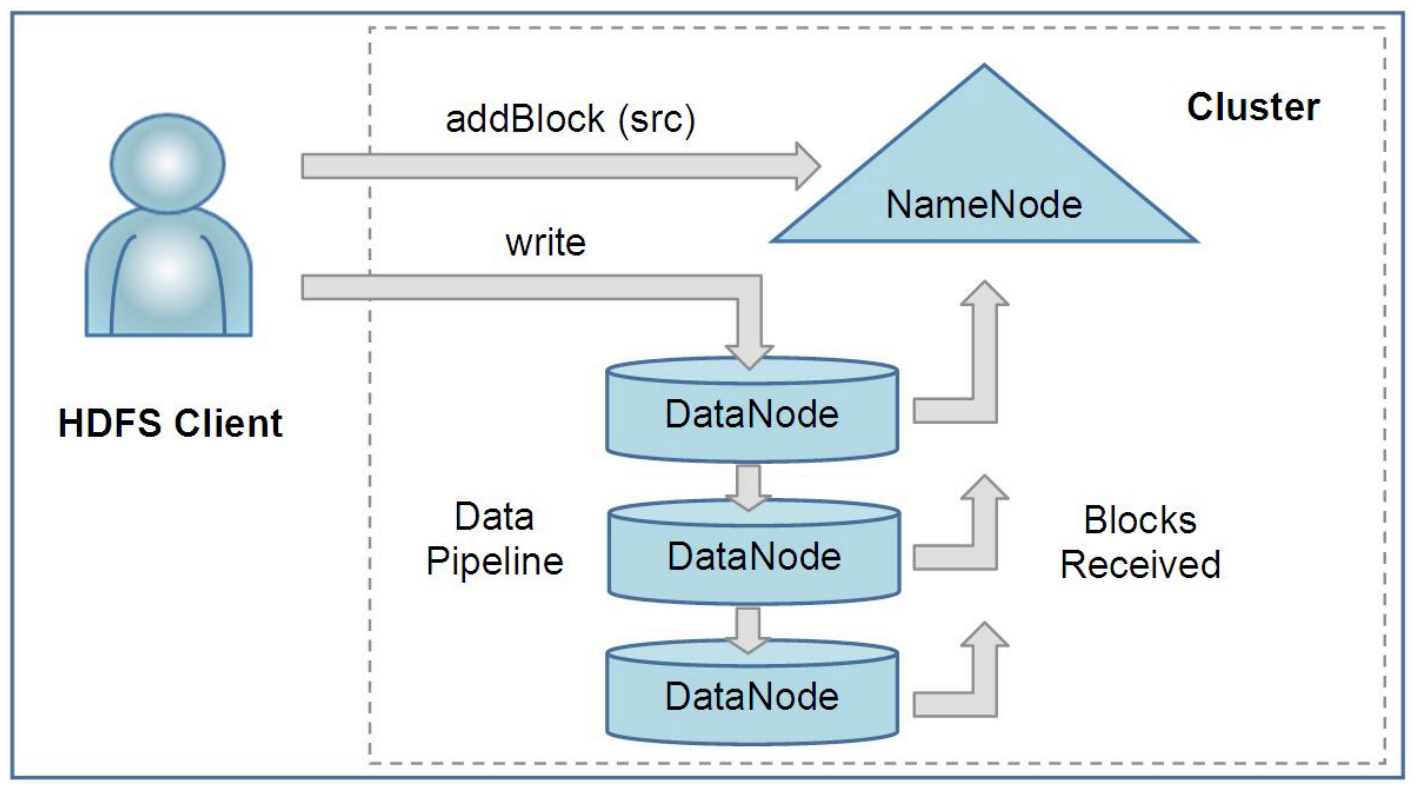
\includegraphics[width=100mm, keepaspectratio]{figures/hdfs_client.png}
	\centering
	\caption*{HDFS file writing}
\end{figure}
The client creates a new file by giving its path to the NameNode. For each block, the NameNode will return a list of DataNodes to place the replicas. The client pipelines data to the given DataNodes, and they will confirm the creation of the block to the NameNode.
\subsection{MapReduce}
MapReduce is a programming model for processing data sets. Users specify two functions \cite{Dean:2004:MSD:1251254.1251264}:
\begin{itemize}
	\item map function: processes a key-value pair to generate a set of key-value pairs
	\item reduce function: merges the intermediate values associated with the same key
\end{itemize}

Programs written in MapReduce are automatically executed parallelly on large clusters. Using this, programmers with no experience in parallel programming and distributed systems can utilize the available resources on the cluster.
\paragraph{Example \cite{MapReduce-example}}
This example shows how MapReduce handles the problem of counting words. We have the following list of words: 
\begin{center}
	\textbf{Dear, Bear, River, Car, Car, River, Deer, Car, Bear}
\end{center}

\begin{figure}[H]
	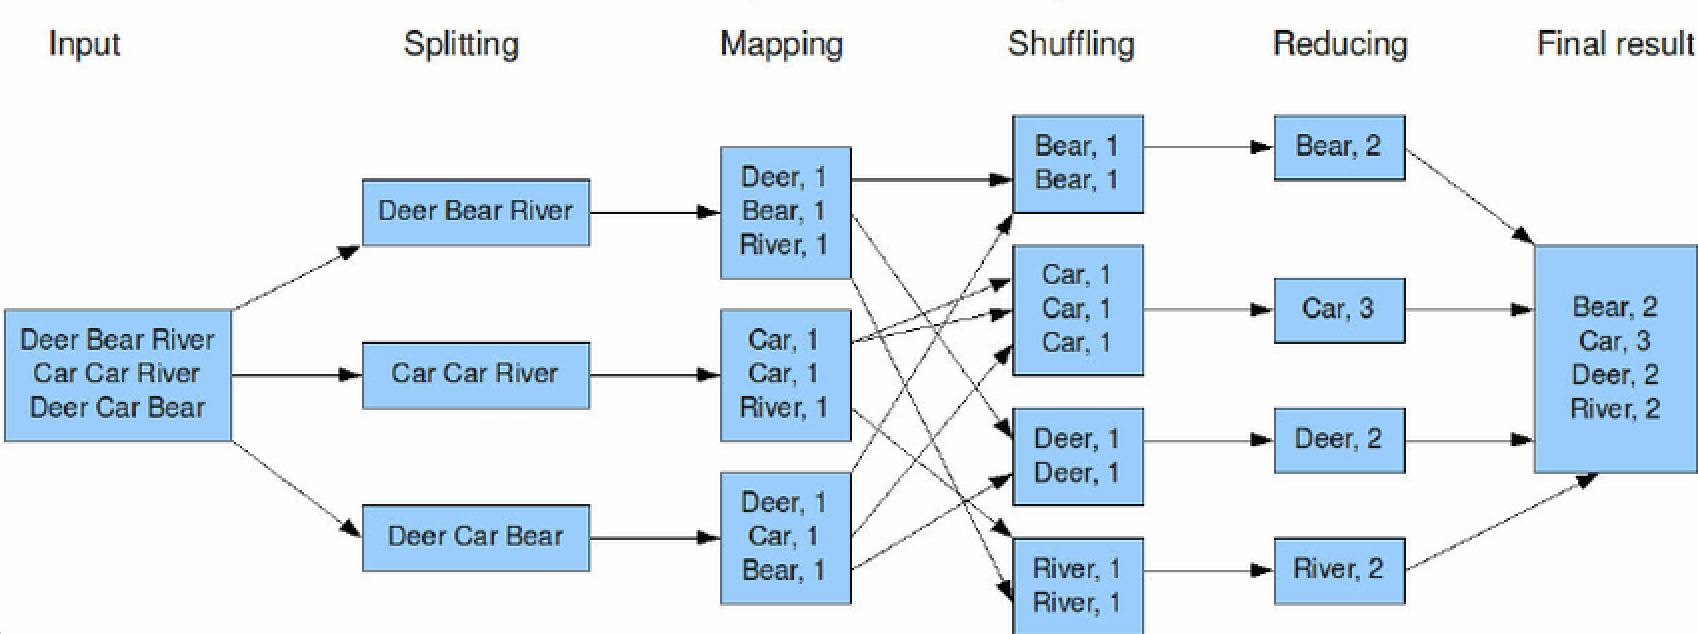
\includegraphics[width=150mm, keepaspectratio]{figures/MapReduce_Example.png}
	\caption*{The MapReduce word count process \cite{MapReduce-example-figure}}
	\centering
\end{figure}
\begin{itemize}
	\item \textbf{Splitting}: the first step is dividing the input into splits. This will distribute the work among the Map nodes.
	\item \textbf{Mapping}: tokenize the words in each mapper and giving a value of 1 for each word, since every word in itself will occur once.
	\item \textbf{Shuffling}: partition takes place with shuffling and sorting: this way pairs with the same key will be sent to the same reducer.
	\item \textbf{Reducing}: a reducer gets the list of pairs and counts the number of ones in this list.
\end{itemize}

\subsubsection*{Advantages of MapReduce \cite{MapReduce-example}}
\paragraph{Parallel processing}
In MapReduce we divide the job among multiple nodes, so they can work on their part of the data parallelly. This way the data processing is done by multiple machines instead of one, so the time is significantly reduced.
\paragraph{Data locality}
In Hadoop MapReduce, instead of moving data into the processing unit, we move the processing unit to the data. The traditional approach has its limit when it comes to processing big data. Moving huge data is costly: network issues can occur and the master node (where data is stored) can get overloaded and may fail. 

However, the MapReduce approach is very cost efficient, since all the nodes are working simultaneously on their part of the data and there is no chance of a node getting overloaded.

Using Hadoop we just need to provide the map and reduce functions, the rest is done by the framework.  The word count example would look like the following in Java:
\paragraph{Map}\mbox{}\\
\begin{lstlisting}[language=Java]
	public void map(LongWritable key, Text value, Context context) throws IOException,InterruptedException {
		String line = value.toString();
		StringTokenizer tokenizer = new StringTokenizer(line);
		while (tokenizer.hasMoreTokens()) {
			value.set(tokenizer.nextToken());
			context.write(value, new IntWritable(1));
		}
	}
\end{lstlisting}
The input and output of the Mapper is a key/value pair. 

Input:
\begin{itemize}
	\item Key: the offset of each line
	\item Value: each line
\end{itemize}

Output:
\begin{itemize}
	\item Key: the tokenized words
	\item Value: the hardcoded value 1
\end{itemize}

\paragraph{Reduce}\mbox{}\\
\begin{lstlisting}
	public void reduce(Text key, Iterable<IntWritable> values,Context context) throws IOException,InterruptedException {
		int sum=0;
		for(IntWritable x: values) {
			sum+=x.get();
		}
		context.write(key, new IntWritable(sum));
	}
\end{lstlisting}
Both the input and output of the Reducer is a key/value pair. 

Input:
\begin{itemize}
	\item Key: unique words, generated after the sorting and shuffling phase
	\item Value: a list of integers corresponding to each keys
	\item \eg Bear, [1, 1]
\end{itemize}

Output:
\begin{itemize}
	\item Key: all the unique words in the input text file
	\item Value: number of occurrences for each unique word
	\item \eg  Bear, 2; Car, 3
\end{itemize}

The traditional way to execute MapReduce operations is that the users specify the Map and Reduce functions in Java. However, this approach has some problems:
\begin{itemize}
	\item it is not a high-level language for data processing
	\item data scientists do not understand Java. They came from the world of traditional databases, where SQL is used.
	\item even a simple problem (like word counting) resulted in hundreds of lines of code.
\end{itemize}

Although, the Hadoop MapReduce framework is written in Java, with the help of Streaming API we can create Map and Reduce functions in any languages.

MapReduce gives us a solution for many big data problems. However, for some scenarios, MapReduce is not the ideal choice: \eg real-time analysis. In Hadoop 1.0 we could not use components other than MapReduce (for example Apache Storm which is ideal for real-time computation). The desire for utilizing the potential provided by the distributed file system (HDFS) in other solutions has grown. YARN provides a solution to fulfill this claim.
\clearpage \subsection{Yarn \cite{YARN}}
\subsubsection*{Hadoop 1.0 resource management}
Previous to Hadoop 2.0, a single JobTracker had the responsibility to monitor the resources and distribute the MapReduce jobs for the DataNodes and monitor these jobs. 

In Hadoop 1.0 the MapReduce module was responsible for cluster resource management and data processing as well.

\begin{figure}[H]
	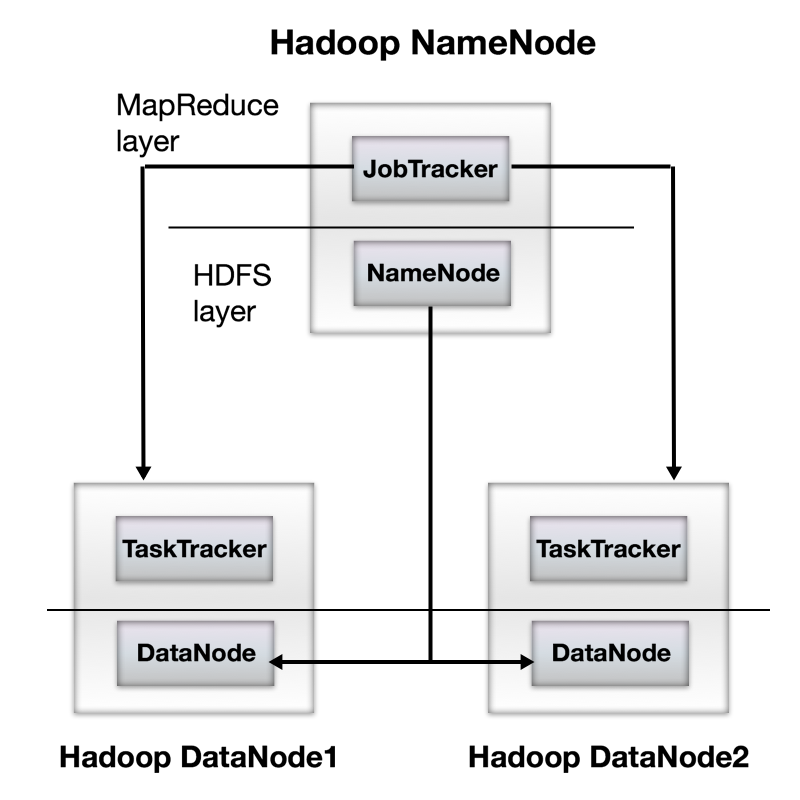
\includegraphics[width=100mm, keepaspectratio]{figures/hadoop10.png}
	\centering
	\caption*{Hadoop 1.0 architecture\cite{Hadoop1.0-problems}}
	\centering
\end{figure}

Resource management in Hadoop 1.0 \cite{Hadoop1.0}:

Clients submit jobs to the JobTracker which turns to the NameNode. It returns the location of the data. The JobTracker locates TaskTracker nodes with available slots close to the data and sends the job to the chosen TaskTracker nodes. After the job has started the JobTracker monitors the chosen TaskTracker nodes. If they do not send heartbeats frequently, they are deemed to have failed so the task will be scheduled on a different TaskTracker. The JobTracker gets a notification if a task fails. It decides what to do then: it may send the job to another TaskTracker, it can mark the record as something to avoid, or it may even put the TaskTracker to blacklist since it is unreliable. If the JobTracker sees that the task is finished, it will update its status. Clients poll the JobTracker for information.

The architecture of Hadoop 1.0 has many problems \cite{Hadoop1.0-problems}:
\begin{itemize}
	\item  It \textbf{limits scalability} since the JobTracker runs on a single machine doing multiple tasks it becomes a bottleneck: resource management, job and task scheduling, monitoring are done by the JobTracker.
	\item JobTracker is a \textbf{Single Point of Failure}. If it goes down, all the jobs are halted.
	\item In Hadoop 1.0 \textbf{JobTracker is tightly integrated with the MapReduce} module so only MapReduce applications can run on Hadoop. Although MapReduce is powerful enough to express many data analysis algorithms (mostly batch-driven data analysis), it is not always the optimal paradigm. It is often desirable to run other computation paradigms on Hadoop like real-time analysis and Message-Passing approach, \etc. Since HDFS makes it easy to store large amounts of data it is desirable to utilize this for other big data problems.
\end{itemize}

Developers recognized that splitting the responsibility to resource management and application monitoring has serious benefits. YARN is a re-architecture of Hadoop that allows multiple applications to run on the same platform. With YARN, applications run "in" Hadoop, instead of "on" Hadoop. This takes Hadoop beyond a batch processing application to a "data operating system" where HDFS is the file system and YARN is the operating system. 

\begin{figure}[H]
	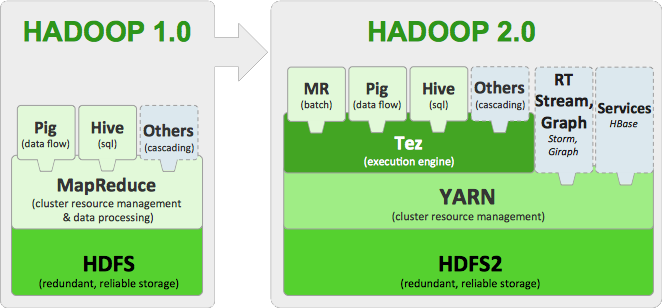
\includegraphics[width=100mm, keepaspectratio]{figures/hadoop10vs20.png}
	\centering
	\caption*{From Hadoop 1.0 to Hadoop 2.0}
	\centering
\end{figure}

The fundamental idea behind YARN is to split up the functionalities of resource management and job scheduling/monitoring. In YARN we have a global ResourceManager (RM) and ApplicationMaster (AM) for each application.

\textbf{ResourceManager} is responsible for distributing the resources among all the applications in the system. The \textbf{NodeManager} is a per-machine agent who monitors the resource usages (CPU, memory, network, disk) of the containers and reports them to the ResourceManager. 

The \textbf{ApplicationMaster} is framework specific, and its task is to ask the ResourceManager for resources when needed. It is also working with the NodeManager to execute and monitor tasks.

The ResourceManager is divided into two main components: Scheduler and ApplicationsManager.
\begin{itemize}
	\item The Scheduler is responsible for allocating resources to applications running in the cluster. It schedules based on the resource requirements of each application. The Scheduler does not perform monitoring or status tracking.
	\item The ApplicationsManager accepts job-submissions. It negotiates the first container for executing the application specific ApplicationMaster. It is also responsible for restarting the ApplicationMaster if it fails. 
\end{itemize}

\begin{figure}[H]
	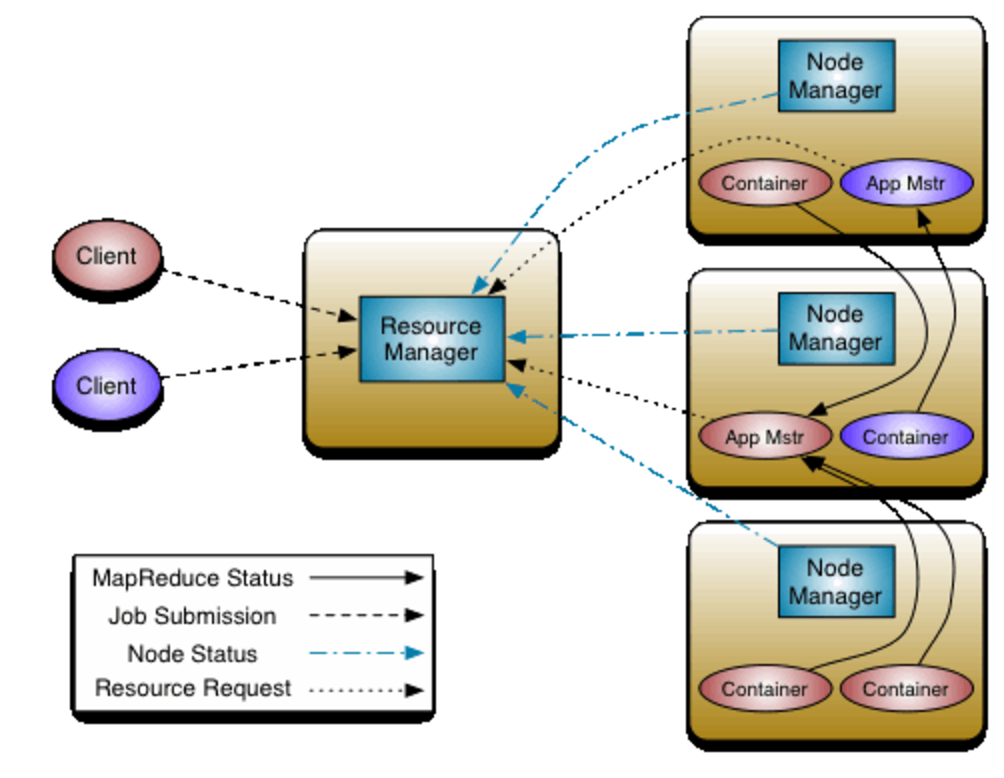
\includegraphics[width=120mm, keepaspectratio]{figures/yarn.png}
	\centering
	\caption*{Yarn architecture}
	\centering
\end{figure}

In summary, with YARN Hadoop is able to run applications that do not follow the MapReduce model since it decouples the resource management and scheduling capabilities of MapReduce. With the help of YARN, we can efficiently utilize the resources and can run multiple applications in Hadoop, all sharing a common resources.

\section{Apache Hive}
Hadoop is a popular implementation of the map-reduce model and used widely to process and store extremely large datasets. However, a map-reduce program is very low level and difficult to maintain or reuse. Data scientist come from a world, where SQL is the standard of data processing. Apache Hive gives us a data warehouse solution built on top of Hadoop to write SQL-like queries so we can utilize the advantage of a declarative language. The language similar to SQL is called HiveQL.

\subsection{Hive \vs RDBMS}
This section shows the main differences between Hive and traditional databases (\eg MySQL, Oracle, MS SQL \etc).

Hive supports SQL interface but it is not a full database. It follows WORM (Write Once Read Many) model while RDBMS is designed for Write and Read many times. Hive uses schema on read and traditional databases offer schema on write. Looking into Hive's approach, data is not validated until it is read. We can define multiple schemas to the same data and it provides a fast initial loading since the operation is just a copy and write. However the schema on read approach has some drawbacks. Schema check on write ensures that the data is not corrupt and it provides a better query performance because when reading data, schema checking is not needed. Hive is a better choice when the schema is not available at loading time since it can be added later dynamically. 

From Hive 0.13, Hive supports transactions \cite{Hive-transactions} and full ACID semantics at row level, but with many limitations. Previous to this, atomicity, consistency and durability were available and only at partition level. With introducing transactions Insert, Update and Delete keywords were added to HiveQL. 

The maximum data size allowed in a traditional RDBMS is 10's of Terabytes. However, Hive can easily handle Petabytes.

\subsubsection*{Conclusion}
Hive is a great choice if we want to analyze large unstructured, relatively static data sets, fast querying is not necessary and easy, low-cost scalability is required. RDBMS provides fast responses for analyzing data dynamically, but scalability and maximum data size are limited.

\subsection{Data storage}
Hive structure data in the following units  \cite{Hive-paper, Hive-data-units}:
\begin{itemize}
\item \textbf{Databases}: namespaces to avoid conflicts of table, partition or bucket names.
\item \textbf{Tables}: storage unit for data with the same schema. Tables maps to directories in HDFS.
\item \textbf{Partitions}: Tables can have many partition keys. These will determine how data is stored. In HDFS partitions map to subdirectories in the table's directory. This way we can speed up the analysis. Instead of running the query in the whole table, Hive will only run our query in the relevant partitions (see example below). Partition columns are virtual, which means they are not part of the data itself.
\item \textbf{Buckets}: Data can be divided into buckets based on the hash value of a column. These are helpful for efficiently sample data. Buckets are stored in files in the table's or partition's directory.
\end{itemize}

\subsubsection*{Example}
This example shows how Hive data units map to HDFS and and how partitioning tables can speed up queries.

Hive tables map to \texttt{<warehouse\_root\_directory>/table\_name} directory. As default, the warehouse root directory is /user/hive/warehouse. This can be changed with the corresponding hive configuration value.
\begin{lstlisting}
	CREATE TABLE test_table(c1 string, c2 int) 
		PARTITIONED BY (date string, hour int);
\end{lstlisting}
The above SQL statement will create a table with two columns and two partitions and it will be stored in  \texttt{/user/hive/warehouse/test\_table} directory in HDFS. For every distinct date and hour value, a partititon will exists. Although, the partition columns are not part of the data, they are stored in the table metadata. 

New partitions can be added either with the INSERT or the ALTER statement. These commands will create the corresponding HDFS directories: 

\texttt{/user/hive/warehouse/test\_table/date=2018-01-01/hour=12 and /user/hive/warehouse/test\_table/date=2018-01-02/hour=11}.

\begin{lstlisting}
	INSERT OVERWRITE TABLE
		test_table PARTITION(date='2018-01-01', hour=12)
	SELECT * FROM t;
	
	ALTER TABLE test_table
		ADD PARTITION(date='2018-01-02', hour=11);
\end{lstlisting}

Hive can use these information for pruning the directories to be scanned for query execution. 
\begin{lstlisting}
	SELECT * FROM test_table WHERE date='2018-01-01';
\end{lstlisting}
In case of this query, Hive will only scan the files in \texttt{/user/hive/warehouse/test\_table/date=2018-01-01} directory. Partitioning our data has significant impact on the time taken by queries.

Although, data in Hive is always in the corresponding directory (\texttt{<warehouse\_root\_directory>/table\_name}), Hive is able to query data stored in other locations in HDFS. In order to do this, we can create EXTERNAL tables as the following statement shows:
\begin{lstlisting}
	CREATE EXTERNAL TABLE test_external(c1 string, c2 int)
		LOCATION '/user/example_table/example_data';
\end{lstlisting}
Hive assumes that the external table in its internal format. The difference between an external and normal (managed by Hive) table is that the drop table command doesn't effect the data itself on an external table. However, on a normal table, it drops the associated data.

\subsection{Architecture}
The main components of Hive are the following \cite{Hive-paper}:
\begin{itemize}
	\item \textbf{Driver}: manages the lifecycle of a HiveQL query by creating a session for it. The driver also collects the result after the execution phase.
	\item  \textbf{MetaStore}: stores metadata about tables, columns or partitions. For example, it stores the table schema and location.
	\item \textbf{Compiler}: compiles the HiveQL statement and generates the execution plan using the partition and table metadata obtained from the MetaStore. First, it parses the query and does semantic analysis. Then converts it into AST (Abstract Syntax Tree) and after compatibility checking to a DAG of Map and Reduce tasks (if Hadoop MapReduce is the execution engine). 
	\item \textbf{Optimizer}: transformations are done to get an optimized DAG for better performance. It is an evolving component. In the earlier stage, only rule-based optimization was available which performed column pruning and predicate pushdown. Later, map-side join was introduced and several other join optimization, also cost-based optimization was added.
	\item \textbf{Execution Engine}: executes the plan created by the compiler. The plan is a DAG of stages. The engine manages the dependencies between these stages and executes them in the corresponding component. Hive is compatible with 3 execution engines: MapReduce, Apache TEZ and Spark which can run in Hadoop YARN.
	\item \textbf{HiveServer2}: a service that provides a thrift interface so clients can execute queries against Hive. Thrift is an RPC (Remote Call Procedure) framework for defining services for multiple languages.
	\item \textbf{Clients}: multiple clients are available to interact with Hive. Beeline (CLI), JDBC/ODBC, Python or Ruby client \etc.
\end{itemize}

\begin{figure}[H]
	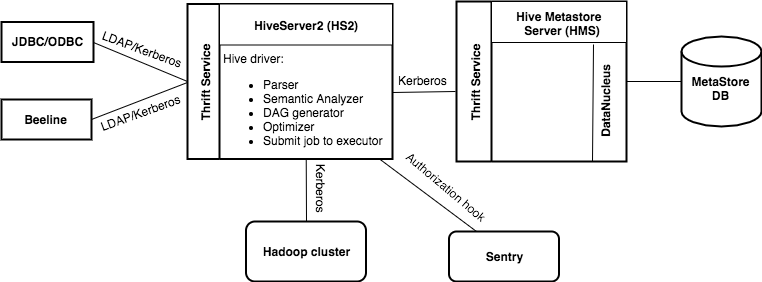
\includegraphics[width=150mm, keepaspectratio]{figures/Hive_architecture.png}
	\centering
	\caption*{Hive architecture}
\end{figure}

Clients can connect to HiveServer2 using its Thrift Service. HS2 supports authentication of the clients using Kerberos or LDAP authentication. Hive Metastore server also supports Kerberos authentication for Thrift clients.

Sentry is a role-based authorization module for Hadoop, so we can control the priviliges for authenticated users. Hive can use Sentry over an "authorization hook", which Sentry registers to Hive configuration file if secure cluster is enabled. 

HMS uses DataNucleus to persist metadata, so any relational database supported by it cal be used: it can be either embedded (\eg Derby) or remote (\eg MySQL) Metastore database.
\include{content/latex-tools}
\include{content/thesis-format}
\include{content/template-usage}


% Acknowledgements
%~~~~~~~~~~~~~~~~~~~~~~~~~~~~~~~~~~~~~~~~~~~~~~~~~~~~~~~~~~~~~~~~~~~~~~~~~~~~~~~~~~~~~~
%----------------------------------------------------------------------------
\chapter*{\koszonetnyilvanitas}\addcontentsline{toc}{chapter}{\koszonetnyilvanitas}
%----------------------------------------------------------------------------

I would like to thank Cloudera Hungary for providing infrastructure and resources for writing my thesis. Especially, I would like thank to the Budapest Hive team for answering my questions and giving all the help they could.

A munka a 2017-1.3.1-VKE-2017-00015 számú projekt keretén belül a Nemzeti Kutatási Fejlesztési és Innovációs Alapból biztosított támogatással, a 2017-1.3. pályázati program finanszírozásában valósult meg.


% List of Figures, Tables
%~~~~~~~~~~~~~~~~~~~~~~~~~~~~~~~~~~~~~~~~~~~~~~~~~~~~~~~~~~~~~~~~~~~~~~~~~~~~~~~~~~~~~~
%\listoffigures\addcontentsline{toc}{chapter}{\listfigurename}
%\listoftables\addcontentsline{toc}{chapter}{\listtablename}


% Bibliography
%~~~~~~~~~~~~~~~~~~~~~~~~~~~~~~~~~~~~~~~~~~~~~~~~~~~~~~~~~~~~~~~~~~~~~~~~~~~~~~~~~~~~~~
\addcontentsline{toc}{chapter}{\bibname}
\bibliography{bib/mybib}


% Appendix
%~~~~~~~~~~~~~~~~~~~~~~~~~~~~~~~~~~~~~~~~~~~~~~~~~~~~~~~~~~~~~~~~~~~~~~~~~~~~~~~~~~~~~~
\include{content/appendices}

%\label{page:last}
\end{document}
